
Foram criadas cinco tabelas relacionadas entre si, conforme ilustrado na \textbf{Figura \ref{fig:conceitual} (p. \pageref{fig:conceitual})}.

Nesse subcapítulo daremos mais atenção à tabela \texttt{Consultas}, pois com ela podemos abordar elementos encontrados nas demais. Nela também adicionamos \texttt{CONSTRAINTS} por fins didáticos, pois, em ambos os casos de uso, seria mais efetivo\footnote{Numa situação de pequenos banco de dados com baixo volume de \texttt{INSERT} e \texttt{UPDATE}, pois \texttt{TRIGGERS} funcionam de forma procedural\cite{TRIGGER_PROC}.} aplicar apenas o uso de \texttt{TRIGGERS}. Veja o script abaixo:

\begin{lstlisting}[
    language=MySQL,
    caption={CREATE TABLE Consultas},
    label=lst:create-consultas-table
]
CREATE TABLE Consultas (
    id_consulta         INT PRIMARY KEY AUTO_INCREMENT,
    id_paciente         INT NOT NULL, 
    id_medico           INT NOT NULL,
    data_consulta       DATE NOT NULL, -- YYYY-MM-DD
    hora_inicio         TIME NOT NULL, -- hh:mm:ss
    hora_fim            TIME NOT NULL, -- hh:mm:ss
    status_consulta     VARCHAR(30), -- confirmado, cancelado, realizado, paci_ausente             

    CONSTRAINT chk_horario_valido CHECK 
        (hora_inicio >= '8:00:00' AND hora_inicio <= '17:00:00'),
    CONSTRAINT chk_horario_fim_valido CHECK 
        (hora_fim > hora_inicio AND hora_fim <= '18:00:00'),

    CONSTRAINT chk_status CHECK 
        (status_consulta IN ('confirmado', 'cancelado', 'realizado', 'paci_ausente')), -- apenas 4 valores são aceitos

    FOREIGN KEY(id_paciente) REFERENCES Pacientes(id_paciente) 
        ON UPDATE CASCADE 
        ON DELETE RESTRICT,
    FOREIGN KEY(id_medico) REFERENCES Medicos(id_medico) 
        ON UPDATE CASCADE 
        ON DELETE RESTRICT
);
\end{lstlisting}
\noindent

\subsubsection{Data Type} % DATA TYPE

A partir da linha 6 é possível perceber que 2 novos tipo de dados são usados, são eles:

\begin{enumerate}
    \item \texttt{DATE} - Uma data. O intervalo suportado é de \texttt{1000-01-01} até \texttt{9999-12-31}. O formato apresentado pelo MySQL para dados do tipo \texttt{DATE} é \texttt{YY-MM-DD} \cite{MySQL_DATE}.
    \item \texttt{TIME} - Um horário. O Intervalo suportado é de \texttt{-838:59:59.000000} até \texttt{838:59:59.000000}. O formato apresentado pelo MySQL para dados do tipo \texttt{TIME} é \texttt{hh:mm:ss} \cite{MySQL_DATE}.
\end{enumerate}

\subsubsection{CONSTRAINT} % CONTRAINT

Já da linha 10 até a linha 16 declaramos nossas \texttt{CONSTRAINT}. Aqui elas têm o papel de impedir que dados inválidos sejam inseridos.
\begin{itemize}
    \item \textbf{Linha 10 e 11} - Valida se o agendamento está sendo feito em horário de funcionamento da clínica.
    \item \textbf{Linha 12 e 13} - Valida se o horário estimado para o fim da consulta faz sentido, isto é, é depois do horário do início e deve ainda estar dentro do horário de funcionamento da clínica.
    \item \textbf{Linha 15 e 16} - Permite apenas 4 tipos de status para consultas, são eles:
        \begin{itemize}
            \item confirmado,
            \item cancelado,
            \item realizado,
            \item paci\_ausente 
        \end{itemize}
\end{itemize}


\subsubsection{Chave Estrangeiras} % CHAVE ESTRANGEIRA

Finalmente, das linhas 18 até a 23 referenciamos nossas chaves estrangeiras.

Assim, temos \texttt{id\_paciente} referenciado da tabela \texttt{Pacientes} e \texttt{id\_medico} referenciado da tabela \texttt{Medicos} respectivamente (\textbf{Figura \ref{fig:conceitual} p. \pageref{fig:conceitual}}). Temos duas opções adicionais para as chaves estrangeiras, são elas:
\begin{itemize}
    \item \textbf{CASCADE} - Seu papel é simples mas crucial. A opção \texttt{CASCADE} faz com que ações tomadas\footnote{Podem ser exclusão (\texttt{ON DELETE}) ou atualização (\texttt{ON UPDATE})} no registro da tabela pai sejam herdadas para todas as colunas filhas que possuem essa opção\cite{delete_cascade}. Aqui usamos \texttt{ON UPDATE}. Portanto, ao atualizar a chave pai, a chave herdada será também excluída.
    % 
    \item \textbf{RESTRICT} - Impede que ocorra a exclusão ou a atualização de um registro da tabela pai, caso ainda hajam registros na tabela filha. Uma exceção de violação de chave estrangeira é retornada. A verificação de integridade referencial é realizada antes de tentar executar a instrução \texttt{UPDATE} ou \texttt{DELETE}\cite{delete_cascade}.
    No script \ref{lst:create-consultas-table} usamos \texttt{ON DELETE}, logo, impedimos que o médico ou paciente seja excluído se ainda houver alguma consulta marcada.
\end{itemize}

\subsection{Alterações}

Podemos alterar colunas com o seguinte script:

\begin{lstlisting}[
    language=MySQL,
    caption=Alter Table,
    label=lst:alterTable
]
ALTER TABLE Prontuarios ADD validade DATE NOT NULL;
ALTER TABLE Prontuarios DROP COLUMN validade;  
\end{lstlisting}

Aqui na linha 1 adicionamos uma coluna do tipo \texttt{DATE} na tabela Prontuário, já na tabela 2 a excluímos. Podemos verificar através do comando \texttt{DESCRIBE}:

\begin{figure}[H]
    \centering
    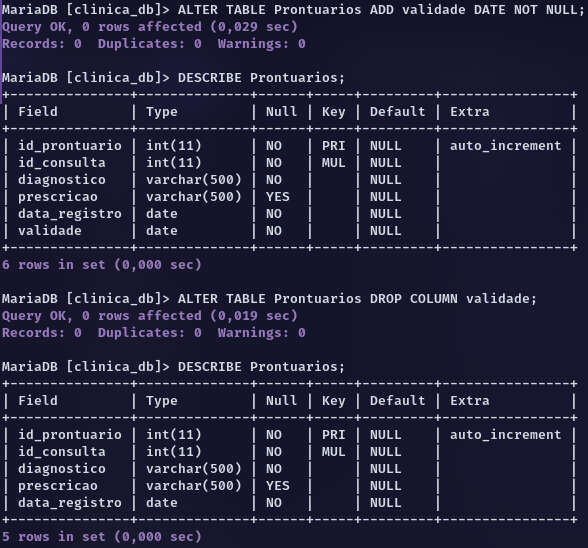
\includegraphics[width=0.85\linewidth]{Text/DDL/Describe.png}
    \caption{Alterações na tabela Prontuários}
    \label{fig:Describe}
\end{figure}

É possível também deletar tabelas no banco de dados com um simples \texttt{DROP TABLES}:

\begin{lstlisting}[
    language=MySQL,
    caption=Alter Table,
    label=lst:alterTable
]
CREATE TABLE teste (coluna_1 INT);
DROP TABLE teste;
\end{lstlisting}

O resultado pode ser visto a seguir:

\begin{figure}[H]
    \centering
    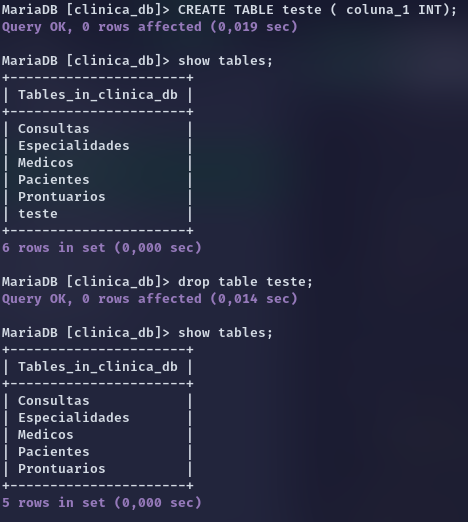
\includegraphics[width=0.50\linewidth]{Text/DDL/drop_table.png}
    \caption{Criação e Exclusão de tabela teste}
    \label{fig:drop_table}
\end{figure}